\documentclass{standalone}
\usepackage{tikz}

\begin{document}

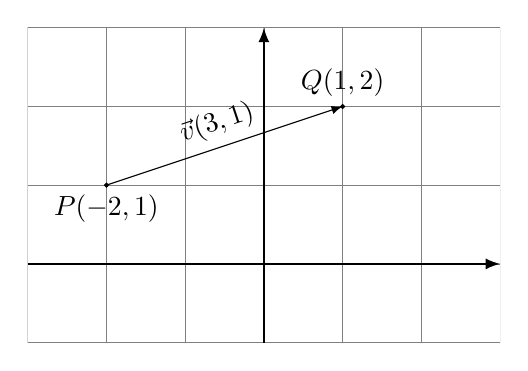
\begin{tikzpicture}
  \path[use as bounding box,clip] (-3,-1) rectangle (3,3);
  \draw[help lines] (-5,-5) grid (5,5);
  \draw[thick,-latex] (-3,0) -- (3,0);
  \draw[thick,-latex] (0,-3) -- (0,3);

  \coordinate (p1) at (-2,1);
  \coordinate (p2) at (1,2);
  \draw[fill=black] (p1) circle [radius=.025cm] node[below] {$P(-2,1)$};
  \draw[fill=black] (p2) circle [radius=.025cm] node[above] {$Q(1,2)$};
  \draw[-latex] (p1) -- (p2) node[midway,above,sloped] {$\vec v(3,1)$};
\end{tikzpicture}

\end{document}